\documentclass[11pt]{scrartcl}

\usepackage[top=1.5cm]{geometry}
\usepackage{url}
\usepackage{float}
\usepackage{listings}
\usepackage{xcolor}
\usepackage{graphicx}
\usepackage{booktabs}

\setlength{\parindent}{0em}
\setlength{\parskip}{0.5em}

\newcommand{\youranswerhere}{[Your answer goes here \ldots]}
\renewcommand{\thesubsection}{\arabic{subsection}}

\lstdefinestyle{dmrsql}{
  language=SQL,
  basicstyle=\small\ttfamily,
  keywordstyle=\color{magenta!75!black},
  stringstyle=\color{green!50!black},
  showspaces=false,
  showstringspaces=false,
  commentstyle=\color{gray}}

\lstdefinestyle{dmrJava}{
  language=JAVA,
  basicstyle=\small\ttfamily,
  keywordstyle=\color{magenta!75!black},
  stringstyle=\color{green!50!black},
  showspaces=false,
  showstringspaces=false,
  commentstyle=\color{gray}}

\title{
  \textbf{\large Projektaufgabe 3 } \\
  Phase 2 – Implementierung des XPath Accelerators (5 P) \\
  {\large Datenmanagement jenseits von Relationen}
}

\author{
  Gruppe A17 \\
  \large Acikyol Aleyna, 12032843 \\
  \large Özcan Ahmet, 12311287 \\
  \large Sadykova Nargiz, 12129337
}

\begin{document}

\maketitle\thispagestyle{empty}

Dieses Reporting Template dient der Vorbereitung der Abgabe von Phase 2.

\subsection*{Verwendung der Daten aus der DBLP (1 Punkt)}

Die DBLP-Daten wurden von \url{https://dblp.org/xml/dblp.xml.gz} heruntergeladen (ca.\ 4\,GB nach dem Entpacken).
Für die speichereffiziente Verarbeitung der großen XML-Datei wurde \texttt{lxml.etree.iterparse}
verwendet, das Datensätze (\texttt{article}, \texttt{inproceedings}) Stück für Stück liest und
verarbeitete Elemente sofort aus dem Arbeitsspeicher entfernt.

Venue-Zuordnung erfolgt ausschließlich anhand des \texttt{key}-Attributs:
\begin{itemize}
  \item \texttt{journals/pvldb/} oder \texttt{conf/vldb/} $\Rightarrow$ \textbf{VLDB}
  \item \texttt{journals/pacmmod/} oder \texttt{conf/sigmod/} $\Rightarrow$ \textbf{SIGMOD}
  \item \texttt{conf/icde/} $\Rightarrow$ \textbf{ICDE}
\end{itemize}

Das Extraktions-Skript \texttt{phase2\_extract\_dblp.py} schreibt alle gefundenen Datensätze
in \texttt{my\_small\_bib.xml} (Wurzelknoten \texttt{bib}, identisches Format wie \texttt{toy\_example.txt}).

Geben Sie die folgende Kennzahl bezogen auf \texttt{my\_small\_bib.xml} an:

\begin{itemize}
  \item Anzahl Publikationen von \textit{Nikolaus Augsten}%
    \footnote{Korrektheit und Vollständigkeit: \url{https://dblp.org/pid/76/3961.html}.}
    \begin{itemize}
      \item ICDE:   \textbf{8}
      \item VLDB:   \textbf{8}
      \item SIGMOD: \textbf{6}
    \end{itemize}
  \item Position (Zeilennummer von\,--\,bis) der Toy-Beispiel-Publikationen in \texttt{my\_small\_bib.xml}
    \begin{itemize}
      \item \texttt{SchmittKAMM23}: \textbf{Zeile 317184--317200}
      \item \texttt{HutterAK0L22}:  \textbf{Zeile 25126--25140}
      \item \texttt{SchalerHS23}:   \textbf{Zeile 306203--306216}
      \item \texttt{ThielKAHMS23}:  \textbf{Zeile 389884--389899}
    \end{itemize}
  \item Dateigröße von \texttt{my\_small\_bib.xml} in kB und Zeilenanzahl:
        \textbf{15\,360\,kB (15\,MB), 391\,821 Zeilen} (22\,691 Publikationen: 8\,014 VLDB, 6\,818 SIGMOD, 7\,859 ICDE)
\end{itemize}

\textbf{Korrektheitsprüfung:} Das Skript gibt nach der Extraktion automatisch aus, ob alle vier
Toy-Beispiel-Artikel (\texttt{SchmittKAMM23}, \texttt{HutterAK0L22}, \texttt{ThielKAHMS23},
\texttt{SchalerHS23}) in \texttt{my\_small\_bib.xml} enthalten sind.

\subsubsection*{Transformation und Import ins EDGE-Modell (0,5 Punkte)}

Das Skript \texttt{phase2\_edge\_import.py} liest \texttt{my\_small\_bib.xml} und baut
daraus denselben EDGE-Baum auf wie in Phase~1 (Wurzel \texttt{bib} $\to$ Venue $\to$
Jahr $\to$ Publikation $\to$ Felder). Der Import nutzt dieselben Tabellen \texttt{node}
und \texttt{edge} aus Phase~1:

\begin{lstlisting}[style=dmrsql, frame=single]
CREATE TABLE node (
    id      SERIAL PRIMARY KEY,
    s_id    VARCHAR,
    type    VARCHAR NOT NULL,
    content TEXT
);

CREATE TABLE edge (
    "from"  INTEGER NOT NULL REFERENCES node(id),
    "to"    INTEGER NOT NULL REFERENCES node(id),
    PRIMARY KEY ("from", "to")
);
\end{lstlisting}

Anzahl der Tupel nach dem Import:
\begin{itemize}
  \item Relation \texttt{node}: \textbf{290\,080}
  \item Relation \texttt{edge}: \textbf{290\,079}
\end{itemize}



\subsection*{Schemaerstellung (1 Punkt).}
Geben Sie die Create Table statements aller von Ihnen angelegten Tabellen an:
\begin{lstlisting}[style=dmrsql]
postgres=# CREATE TABLE accel (
  pre    INTEGER,
  post   INTEGER,
  parent INTEGER,
  kind   TEXT,
  name   TEXT
);

CREATE TABLE content (
  pre  INTEGER,
  text TEXT
);
CREATE TABLE
CREATE TABLE
postgres=# CREATE TABLE attribute ( pre  INTEGER,
  text TEXT
);
\end{lstlisting}

\subsection*{Pre-/Post-Order Annotation (1 Punkt).}
Definieren Sie sich einen \textit{Ausschnitt} aus \texttt{toy\_example.txt}. Berechnen Sie hierfür händisch die Pre-/Post-Order Annotation. Inkludieren Sie diese als Foto / Screenshot oder ähnliches in dieses Dokument. Zeigen Sie dann, dass Ihre Lösung hierfür dieselben Ergebnisse liefert. Sie können Die Mittels Foto / Screenshot belegen oder in der Übung zeigen.

Ausschnitt aus toy_example.txt:
<bib>
	<article mdate="2024-02-05" key="journals/pvldb/SchmittKAMM23">
		<author orcid="0009-0005-7656-7526">Daniel Ulrich Schmitt</author>
		<author>Daniel Kocher</author>
		<author orcid="0000-0002-3036-6201">Nikolaus Augsten</author>
		<author>Willi Mann</author>
		<author>Alexander Miller</author>
		<title>A Two-Level Signature Scheme for Stable Set Similarity Joins.</title>
		<pages>2686-2698</pages>
		<year>2023</year>
		<volume>16</volume>
		<journal>Proc. VLDB Endow.</journal>
		<number>11</number>
		<ee type="oa">https://www.vldb.org/pvldb/vol16/p2686-schmitt.pdf</ee>
		<ee>https://doi.org/10.14778/3611479.3611480</ee>
		<url>db/journals/pvldb/pvldb16.html#SchmittKAMM23</url>
	</article>
	
\begin{figure}[H]
  \centering
  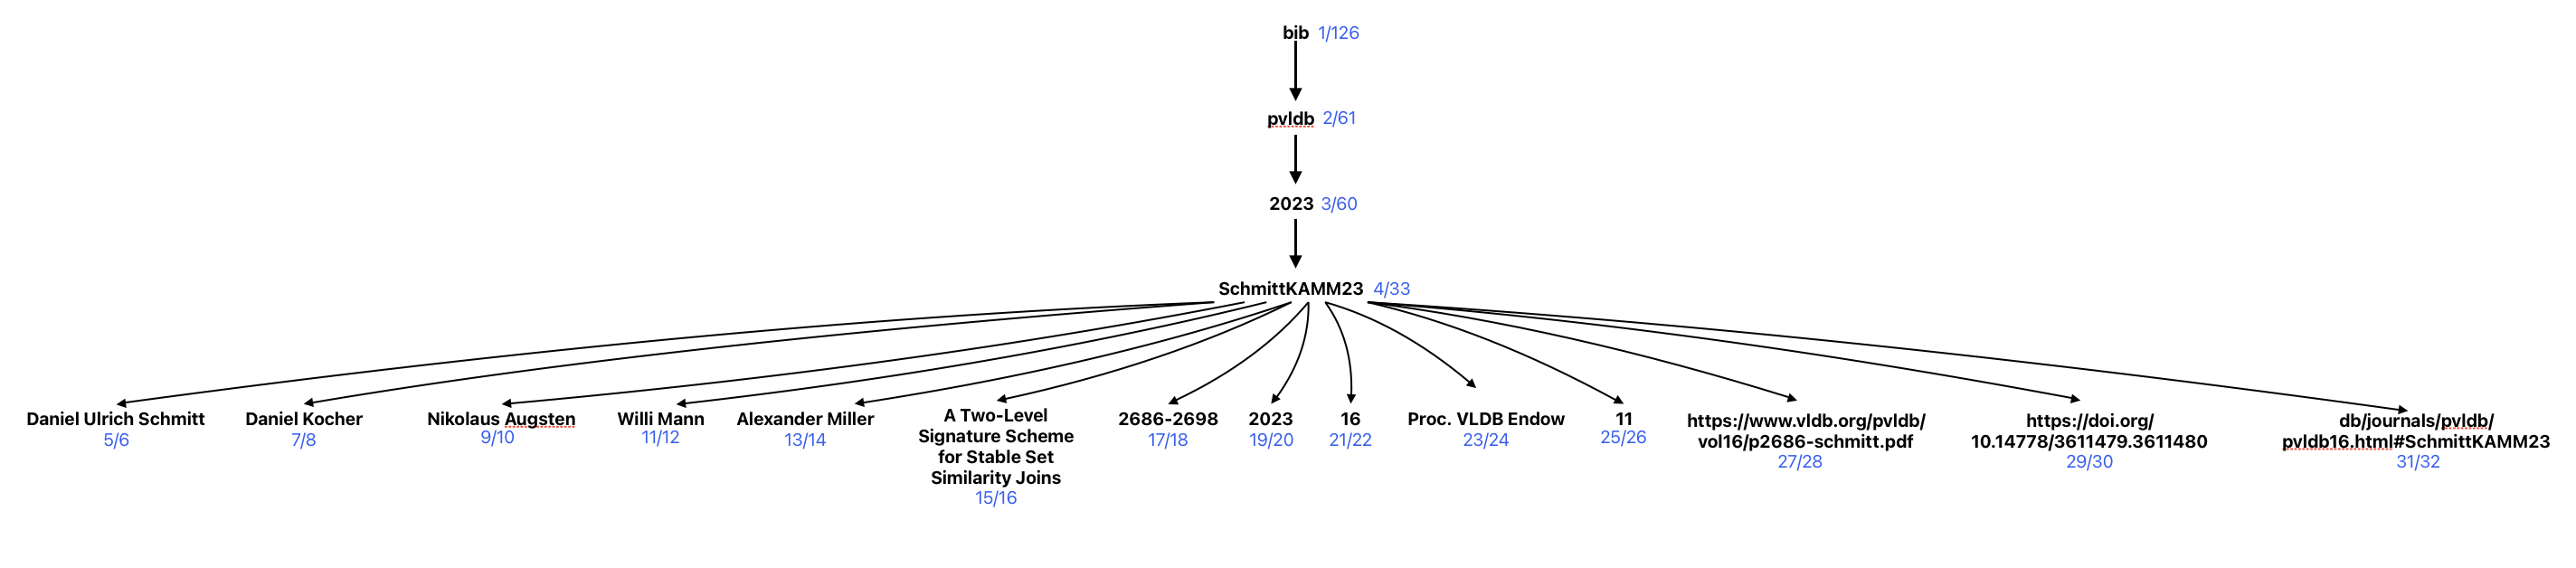
\includegraphics[width=0.8\textwidth]{annotatedtree.png}
\end{figure}

\subsection*{Achse als Fenster (2 Punkt)}
Zeigen Sie, dass die Berechnung der Achsen für die Beispiele aus Phase 1 hier die gleichen Ergebnisse erzeugen:

\begin{table}[h]
	\centering
		\begin{center}
			\begin{tabular}{ l | c c }
				\toprule
				Achse & Ergebnisknoten ID's & Ergebnisgröße\\
				\midrule
				ancestor & ... & ... \\ 
				descendants & ... & ... \\  
				following SchmittKAMM23& ... & ... \\  
				preceeding SchmittKAMM23 & ... & ... \\ 
				following SchalerHS23& ... & ... \\  
				preceeding SchalerHS23& ... & ... \\ 
				\bottomrule
			\end{tabular}
			\end{center}
	\caption{Ergebnisse der XPath-Berechnung auf Edge Modell aus Phase 1}
	\label{tab:ErgebnisseDerXPathBerechnug}
\end{table}

\begin{table}[h]
	\centering
		\begin{center}
			\begin{tabular}{ l | c c }
				\toprule
				Achse & Ergebnisknoten ID's & Ergebnisgröße\\
				\midrule
				ancestor & ... & ... \\ 
				descendants & ... & ... \\  
				following SchmittKAMM23& ... & ... \\  
				preceeding SchmittKAMM23 & ... & ... \\ 
				following SchalerHS23& ... & ... \\  
				preceeding SchalerHS23& ... & ... \\ 
				\bottomrule
			\end{tabular}
			\end{center}
	\caption{Ergebnisse der XPath-Berechnung des XPath-Accelerators aus Phase 2}
	\label{tab:ErgebnisseDerXPathBerechnug}
\end{table}

\subsection*{Zeitmamagement}

Benötigte Zeit pro Person (nur Phase 2):
\begin{itemize}
  \item \textbf{Acikyol Aleyna:} TODO Std.
  \item \textbf{Özcan Ahmet:} TODO Std.
  \item \textbf{Sadykova Nargiz:} 4.5 Std.
\end{itemize}


\end{document}
